%%%%%%%%%%%%%%%%%%%%%%%%%%%%%%%%%%%
% Main Text
%%%%%%%%%%%%%%%%%%%%%%%%%%%%%%%%%%%
\textbf{ACKNOWLEDGMENT} \\ 
I would like to express my special thanks of gratitude to my teacher, Dr.Nguyen Viet Dung() who gave me the golden support to do this wonderful project. He gave a chance to use High GPU computing computer for AI Training. Otherwise, he also gave me recommendation on how to implement experiment to make a good conclusion such as what I should focus on, what I need to investigate, which metrics I should consider.  
\section{Introduction}
%The Need of AI-enabled computer-aided diagnostics
Skin cancer is one of the most common cancer leading causes of death worldwide. Every day, more than 9500\cite{03358} people in the United States are diagnosed with skin cancer. Otherwise, 3.6\cite{03358} million people are diagnosed with basal cell skin cancer each year. According to the Skin Cancer Foundation, the global incidence of skin cancer continues to increase\cite{11872}. In 2019, it is estimated that 192,310 cases of melanoma will be diagnosed in the United States\cite{11872}. On the other hand, if patients are early diagnosed, the survival rate is correlated with 99\%. However, once disease progresses beyond the skin, survival is poor\cite{11872}. Moreover, with the increasing
incidence of skin cancers, low awareness among a growing population, and a lack of adequate clinical expertise and services, there is a need of effective solution. \newline
%The Need of AI-enabled computer-aided diagnostics in Skin Lesion Clasification
Recently, deep learning particularly, and machine learning in generally algorithms have emerged to achieve excellent performance on various tasks, especially in skin disease diagnosis tasks. AI-enabled computer-aided diagnostics (CAD) has solutions in three main categories: Diagnosis, Prognosis and Medical Treatment. Medical imaging, including ultrasound, computed tomography, and magnetic resonance imaging, and X-ray image is used extensively in clinical practice. In Diagnosis, Artificial Intelligence (AI) algorithms are applied for disease detection to save progress execution before these diagnosed results are considered by a doctor. In Prognosis, AI algorithms are used to predict the survival rate of a patient based on his/her history medical data. In Medical Treatment, AI models are applied for building solution for a specific disease, medicine revolutionize is an example. In various studies, AI algorithms has provided various end-to-end solutions in the detection of abnormalities such as breast cancer, brain tumors, lung cancer, esophageal cancer, skin lesions, and foot ulcers across multiple image modalities of medical imaging\cite{11872}. \\
%The Success in AI - especially in CNN - some model based CNN
In order to adapt the increase in skin cancer case, AI algorithms over the last decade has a great performance. Some typical models that can be mentioned are DenseNet\cite{06993}, EfficientNet\cite{04861}, Inception\cite{00567}, MobileNets\cite{04861}\cite{04381}\cite{02244}, ResNet\cite{03385}\cite{05027}, and NasNet\cite{07012}. Some of these models have been used as a backbone model in other studies that I will discuss more in the Related Work section. \\
In this paper, I will analyze the effect of the metadata on classifying skin disease. On the other hand, by analyzing the combination of several backbone models, I will also construct an optimized model that has ability to classify in a balanced way between classes instead of well identifying the majority of classes. 

\section{Related Work} 

\section{Data}
\subsection{Image Data}
The dataset used in this paper is the HAM10000 dataset published by Havard University Dataverse\cite{10417}. There are total 7 classes in this dataset containing Actinic keratoses and intraepithelial carcinoma or Bowen's disease (AKIEC), Basal cell Carcinoma (BCC),  benign keratosis-like lesions (solar lentigines / seborrheic keratoses andchen-planus like keratoses, BKL), dermatofibroma (DF), melanoma (MEL), melanocytic nevi (NV), and vascular lesions (angiomas, angiokeratomas, pyogenic granulomas and hemorrhage, VASC). The distribution of the dataset is shown in the table below:
\begin{center}
	\begin{tabular}{|c c c c c c c c c|} 
		\hline
		Class & AKIEC & BCC & BKL & DF & MEL & NV & VASC & Total \\ 
		\hline
		No. Sample & 327 & 514 & 1099 & 115 & 1113 & 6705 & 142 & 10015 \\
		\hline
	\end{tabular}
\end{center}
\begin{figure}
	\centering
	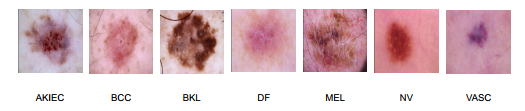
\includegraphics[width=1\linewidth]{img/DataDistribution}
	\caption{Example image of each class}
	\label{fig:datadistribution}
\end{figure}
More than 50 percent of lesions are confirmed through histopathology (HISTO), the ground truth for the rest of the cases is either follow-up examination (FOLLOWUP), expert consensus (CONSENSUS), or confirmation by in-vivo confocal microscopy (CONFOCAL). On the other hand, before being used for training the whole data is shuffled then split into two part. $90$ percent and $10$ percent of the data is used for training and validating respectively.\\
In the previous paper\cite{03358}, the image data is augmented for all class, the number of image increase to 18015 images. Since, this data is imbalanced, using augmented data may cause the problem of well classify on the majority of class. In this paper, instead of augmenting data, metadata is used. The way of processing metadata is discuss in MetaData section. Images in this dataset has the type of $RGB$ and shape of (450, 600). However, Each backbone need the different input size of image as well as the range of pixel value. DenseNet201\cite{06993} require the input pixels values are scaled between $0$ and $1$ and each channel is normalized with respect to the ImageNet dataset. In Resnet50 and Resnet152\cite{03385}\cite{05027}, the images are converted from $RGB$ to $BGR$, then each color channel is zero-centered with respect to the ImageNet dataset, without scaling. InceptionResNetV2\cite{11946}, on the other hand, will scale input pixels between $-1$ and $1$. Similarly, three versions of MobileNet\cite{04861}\cite{04381}\cite{02244}, NasNetMobile and NasNetLarge\cite{07012} require the input pixel is in range of $-1$ and $1$. 
\subsection{Metadata}
The HAM10000 dataset\cite{10417} also contain the metadata of patient including gender, age, and the capturing position. During the data exploration term, I found out that the age category miss 57 data point, then I decided to remove this 57 samples. In the gender and capturing position category contain some samples of unknown. Instead of removing, these unknowns data point is kept and considered as "prefer not to say". Besides, the label of the whole data is preprocessed into one-hot vector.
\section{Model Schema}
\subsection{Input Schema}
%Other preprocessed input%
Using metadata as another input is not new. In paper\cite{03910}, they decide to keep the missing value and set its value to $0$. The sex and anatomical site are categorical encoded. The age, on the other hand is numerical normalized. After processing, the metadata is fed into a two-layer neural network with 256 neurons each. Each layer contains batch normalization, a ReLU\cite{08375} activation and dropout with $p = 0.4$. The network’s output is concatenated with the CNN’s feature vector after global average pooling. Especially, they use a simply data augmentation strategy to address the problem of missing values in metadata. During training, they randomly encode each property as missing with a probability of $p = 0.1$. \\
%My proprocessed input%
In this paper, the unknowns is kept as a type as discussed in Metadata section. Sex, anatomical site and age are also category encoded and numerical normalized, respectively. After processing, the metadata is then concatenated and fed into a dense layer of 4096 neurons. Finally, this this dense layer is then concatenate with the output of Soft-Attention which is then discussed in Soft-Attention section. \\
%Figure%
The Input schema is described as follow:\\
\begin{figure}[h]
	\centering
	\includegraphics[width=0.7\linewidth]{"Diagram/Input Schema"}
	\caption{Input Schema}
	\label{fig:input-schema}
\end{figure}\\
Image data, on the other hand after being preprocessed, is fed directly into the backbone model. 
\subsection{Soft-Attention}
Applying Soft-Attention layer in deep learning is not a new approach. Soft-Attention have been used in various application: image caption generation in \cite{03044} and handwriting verification in \cite{202017} respectively. In skin lesion classification, Soft-Attention is used to increase the performance of the model as described in \cite{03358}. Soft-Attention has ability to ignore irrelevant areas of the image by multiplying the corresponding feature maps with low weights. The function below describe the flow of Soft-Attention module:
\[
	f_{sa} = \gamma t\sum_{k=1}^{K}softmax(W_k * t)
\]
In order to apply Soft-Attention, there are two main steps. Firstly, the input tensor is put in a grid-based feature extraction from the high-resolution image, where each grid cell is analyzed in the whole slide to generate a feature map\cite{08513}. This feature map called $t \in R^{h \times w \times d}$ where $h, w, and d$ is the shape of tensor generate by a Convolution Neural Network(CNN), is then input to a 3D convolution layer whose weights is $W_k \in R^{h \times w \times d \times K}$. The output of this convolution is normalized using softmax function to generate K = 16 attention maps. These $16$ attention maps are aggregated to produce a weight function called $\alpha$. This $\alpha$ function is then multiplied with feature tensor $t$ and scaled by $\gamma$, a learnable scalar. Finally, the out of Soft-Attention function $f_{sa}$ is the concatenation of the beginning feature tensor $t$ and the scaled attention maps. 
\begin{figure}
	\centering
	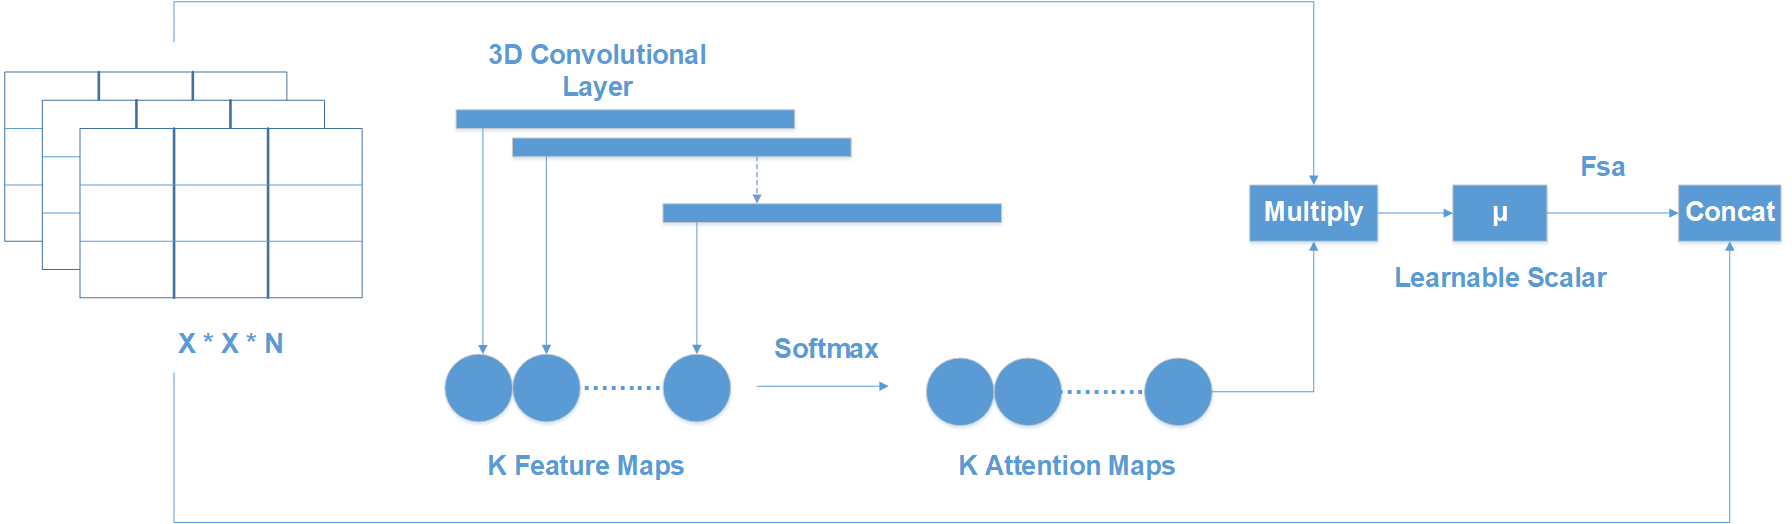
\includegraphics[width=1\linewidth]{Diagram/SoftAttention}
	\caption{Soft-Attention Module}
	\label{fig:softattention}
\end{figure}
In this paper, the Soft-Attention layer is applied in the same way in this paper\cite{03358}. The Soft-Attention module is described in the following diagram:
\begin{figure}[h]
	\centering
	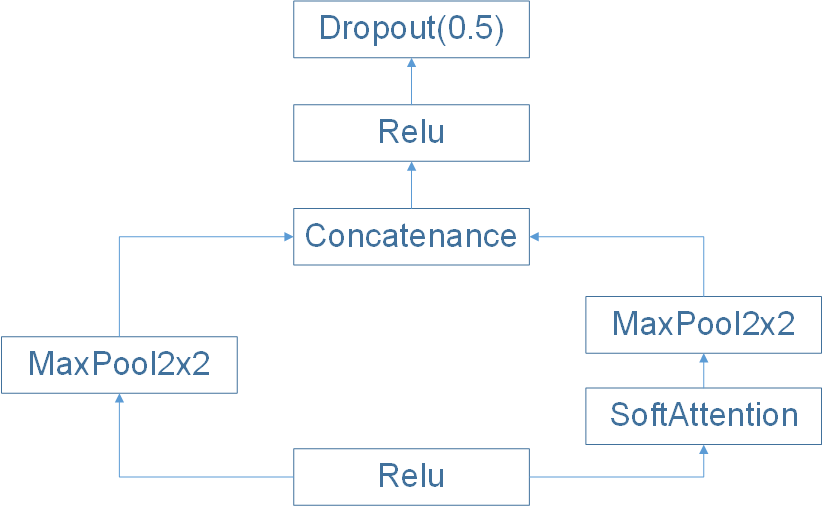
\includegraphics[width=0.5\linewidth]{Diagram/SoftAttentionBlock}
	\caption{Soft-Attention Module}
	\label{fig:softattentionblock}
\end{figure}\\


\subsection{Backbone Model Architecture}
In this paper, the backbone models that have been used are DenseNet201\cite{06993}, Inception\cite{00567}, MobileNets\cite{04861}\cite{04381}\cite{02244}, ResNet\cite{03385}\cite{05027}, and NasNet\cite{07012}. The combination of DenseNet201, InceptionResNetV2 and Soft-Attention layer are both test by the previous paper\cite{03358} with a great performance. Otherwise, Resnet50 also well classify but with much less number of parameter and depth than based on its f1-score and precision stated. Therefore, in this paper, I will analyze the performance of the model Resnet152 and NasnetLarge which has the larger number of parameter and depth. On the other hand, three version of MobileNet and the NasnetMobile will also be analyzed which has a small number of parameter and depth.  
\begin{center}
	\begin{tabular}{|c | c c c|} 
		\hline
		Model & Size(MB) & Parameters & Depth \\ 
		\hline
		Resnet50 & 98 & 25.6M & 107 \\ 
		\hline
		Resnet152 & 232 & 60.4M & 311 \\ 
		\hline
		DenseNet201 & 80 & 20.2M & 402 \\
		\hline
		InceptionResNetV2 & 215 & 55.9M & 449 \\
		\hline
		MobileNet & 16 & 4.3M & 55 \\ 
		\hline
		MobileNetV2 & 14 & 3.5M & 105 \\ 
		\hline
		MobileNetV3Small & Unknown & 2.5M & 88 \\ 
		\hline
		MobileNetV3Large & Unknown & 5.5M & 118 \\
		\hline
		NasnetMobile & 23 & 5.3M & 308 \\
		\hline
		NasnetLarge & 343 & 88.9M & 533 \\ 
		\hline
	\end{tabular}
\end{center}

\subsection{Model}
The whole architecture of the model used for image feature extraction is applied in the same way in paper \cite{03358}. Metadata branch, otherwise is preprocessed before feeding into a dense layer then concatenate with the output of Soft-Attention layer. It is described in the figure below:
\begin{figure}[h]
	\centering
	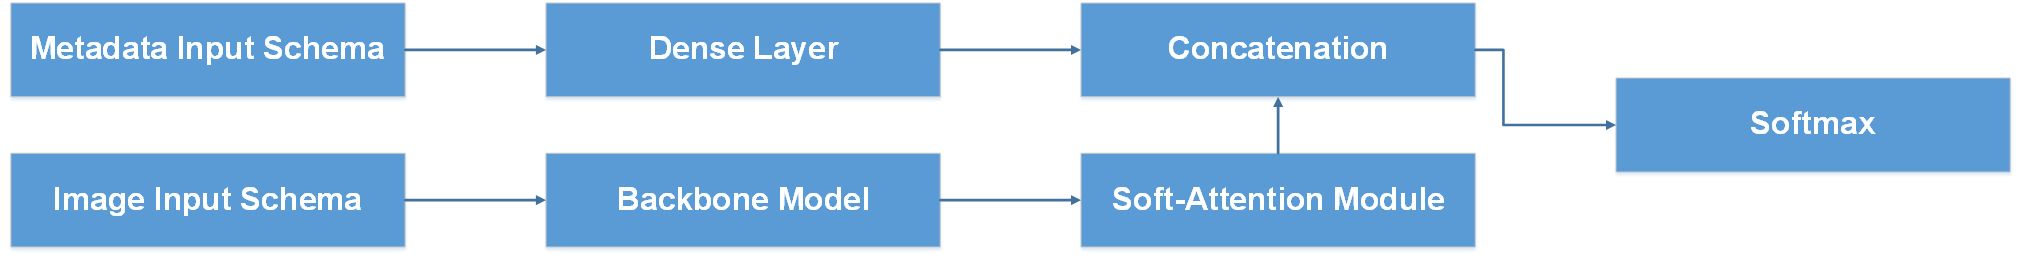
\includegraphics[width=1\linewidth]{Diagram/MainModel}
	\caption{Overall Model}
	\label{fig:mainmodel}
\end{figure}
\section{Training}
\subsection{Loss Function}
The loss function used in this paper is categorical cross-entropy. Consider $X = [x_1, x_2, \dots, x_n]$ as the input feature, $\theta = [\theta_1, \theta_2, \dots, \theta_n]$. Let $N$, and $C$ is the number of training examples and number of class respectively. The categorical cross-entropy loss is presented as:
\[L(\theta, x_n) = -\frac{1}{N}\sum_{c=1}^{C}\sum_{n=1}^{N}y^c_n\log(\hat{y}^c_n)\]
where $\hat{y}^c_i$  is the output of model and $y^c_i$ is the target that the model should return. \\
Since the dataset face the imbalanced problem then I applied the class weight for the loss. This formula below is used to calculate the class weight:
\[W = N \odot D\]
\[D = \begin{bmatrix}
	\frac{1}{C \times  N_1} & \frac{1}{C \times  N_2} & \dots & \frac{1}{C \times  N_n}\\
\end{bmatrix} = \frac{1}{C} \odot \begin{bmatrix}
\frac{1}{N_1} & \frac{1}{N_2} & \dots & \frac{1}{N_n}\\
\end{bmatrix}\]
where $N$ is the number of training sample, $C$ is the number of class, $N_i$ is the number of sample in each class $i$. $D$ is the matrix contain the inverse of $C \times N_i$. The overall loss function is then become\cite{8943952}:
\[
	L(\theta, x_n) = -\frac{1}{N}\sum_{c=1}^{C}\sum_{n=1}^{N} W_c \times y^c_n \times \log(h_\theta(x_n, c))
\]
where $W_c$ is the weight of class $c$, $y^c_n$ is the expected output of class $c$ at training example $n$. Otherwise, $h_\theta$ is the model with weight $\theta$.
\subsection{Evaluation Metrics}
\begin{figure}[!htb]
	\begin{minipage}{0.48\textwidth}
		\centering
		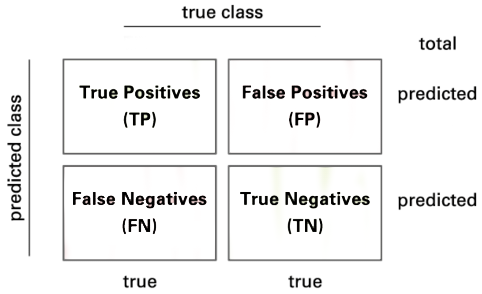
\includegraphics[width=1.1\linewidth]{img/Confusion-matrix}
		\caption{Confusion Matrix}\label{Fig:Data1}
	\end{minipage}\hfill
	\begin{minipage}{0.48\textwidth}
		\centering
		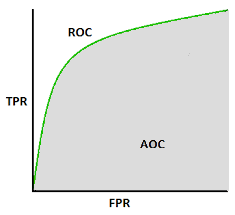
\includegraphics[width=.7\linewidth]{img/AUC}
		\caption{Area Under the Curve}\label{Fig:Data2}
	\end{minipage}
\end{figure}
In this paper, the model is evaluated by using the confusion matrix and related metrics. The figure 4 illustrates the presentation of a $2 \times 2$ confusion matrix used for $2$ class. Consider a confusion matrix $A$ with $C$ number of class. Let $A^i$ and $A^j$ is the set of $A$ rows and columns respectively. 
\[
	A = \begin{bmatrix}
		a_{11} & a_{12} & \dots & a_{1j} \\
		a_{21} & a_{22} & \dots & a_{2j} \\
		\vdots & \vdots	&  & \vdots\\
		a_{i1} & a_{i2} & \dots & a_{ij} 
	\end{bmatrix}
\]
The True Positive(TP) of all class in this case is the main diagonal of the matrix $A$. The following method are used to calculate the False Positives(FP), False Negatives(FN), and True Negatives(TN) of all class:
\[
	FP = -TP + \sum_{k=1}^{i}A^i_k \hspace{1cm} FN = -TP + \sum_{k=1}^{j}A^j_k
\]
\[
	TN_c = \sum_{i=1}^{C}\sum_{j=1}^{C}a_{ij} - \left[ \sum_{k=1}^{i}A^i_{i=c k} + \sum_{k=1}^{j}A^j_{j=c k} \right] + a_{i=c j=c} \implies TN = \begin{bmatrix}
		TN_1 & TN_2 & \dots & TN_c
	\end{bmatrix}
\]
Then, the model is evaluated by the following metrics:
\[\text{Sensitivity(Sens)} = \frac{TP}{TP + FN} \hspace{1cm} \text{Specificity(Spec)} = \frac{TN}{TN + FP}\]
\[\text{Precision} = \frac{TP}{TP + FP} \hspace{1cm} \text{F1 Score} = \frac{2 \times TP}{2 \times TP + FP + FN + TN}\]
\[\text{Accuracy} = \frac{TP + TN}{TP + FP + FN + TN} \hspace{1cm} \text{Balanced Accuracy} = \frac{\text{Sens} + \text{Spec}}{2}\]
The last metric is the $AUC$ score standing for Area Under the Curve which is the Receiver Operating Curve(ROC) that indicate the probability of TP versus the probability of FP.  
\section{Experiment}
All the model in this paper is trained with Adam Optimizer\cite{6980}. The initial learning rate is set to $0.001$, an learning rate reduction schedule is setup with the minimum learning rate is $0.0000001$ with the factor of $0.2$. Otherwise, the epsilon argument of the optimizer is set to $0.1$. The performance of all model is presented in the figure below:
\section{Conclusion}
\clearpage
\pagebreak

